\chapter{Examples}\label{ch:examples}\pagenumbering{arabic}

\todo{Remove this example todo.}

\section{Inline Code, Footnotes and URLs}

This an example text, which shows you, how to use the \texttt{tudscr}\footnote{TUD-Script. \url{https://github.com/tud-cd/tudscr} (Visited on Sept. 15 2020)} template and its components. Feel free to remove this example text or use the provided segments for your thesis.

\section{Research Questions, Inline TODOs, Citations and Referencing}


We'd like to answer the following research goals.\todo[inline]{You may of course write some more text than given in this example.}

\begin{researchquestion}\label{rq:matrix}
Do we live in the Matrix?
\end{researchquestion}

\noindent Feel free to explain the motivation behind your research questions.

\begin{researchquestion}\label{rq:possible}
Based on \cite{gos_2020}, is it actually possible to answer \Cref{rq:matrix} in the first place?
\end{researchquestion}

\noindent This research question is relevant, because it just came to my mind. Pull Request if you have a better example, thanks.

\section{Including Graphics and Paragraphs}

Although this has really nothing to do with the previous sections, take the following as an example of how to include graphics.

\begin{figure}[H]
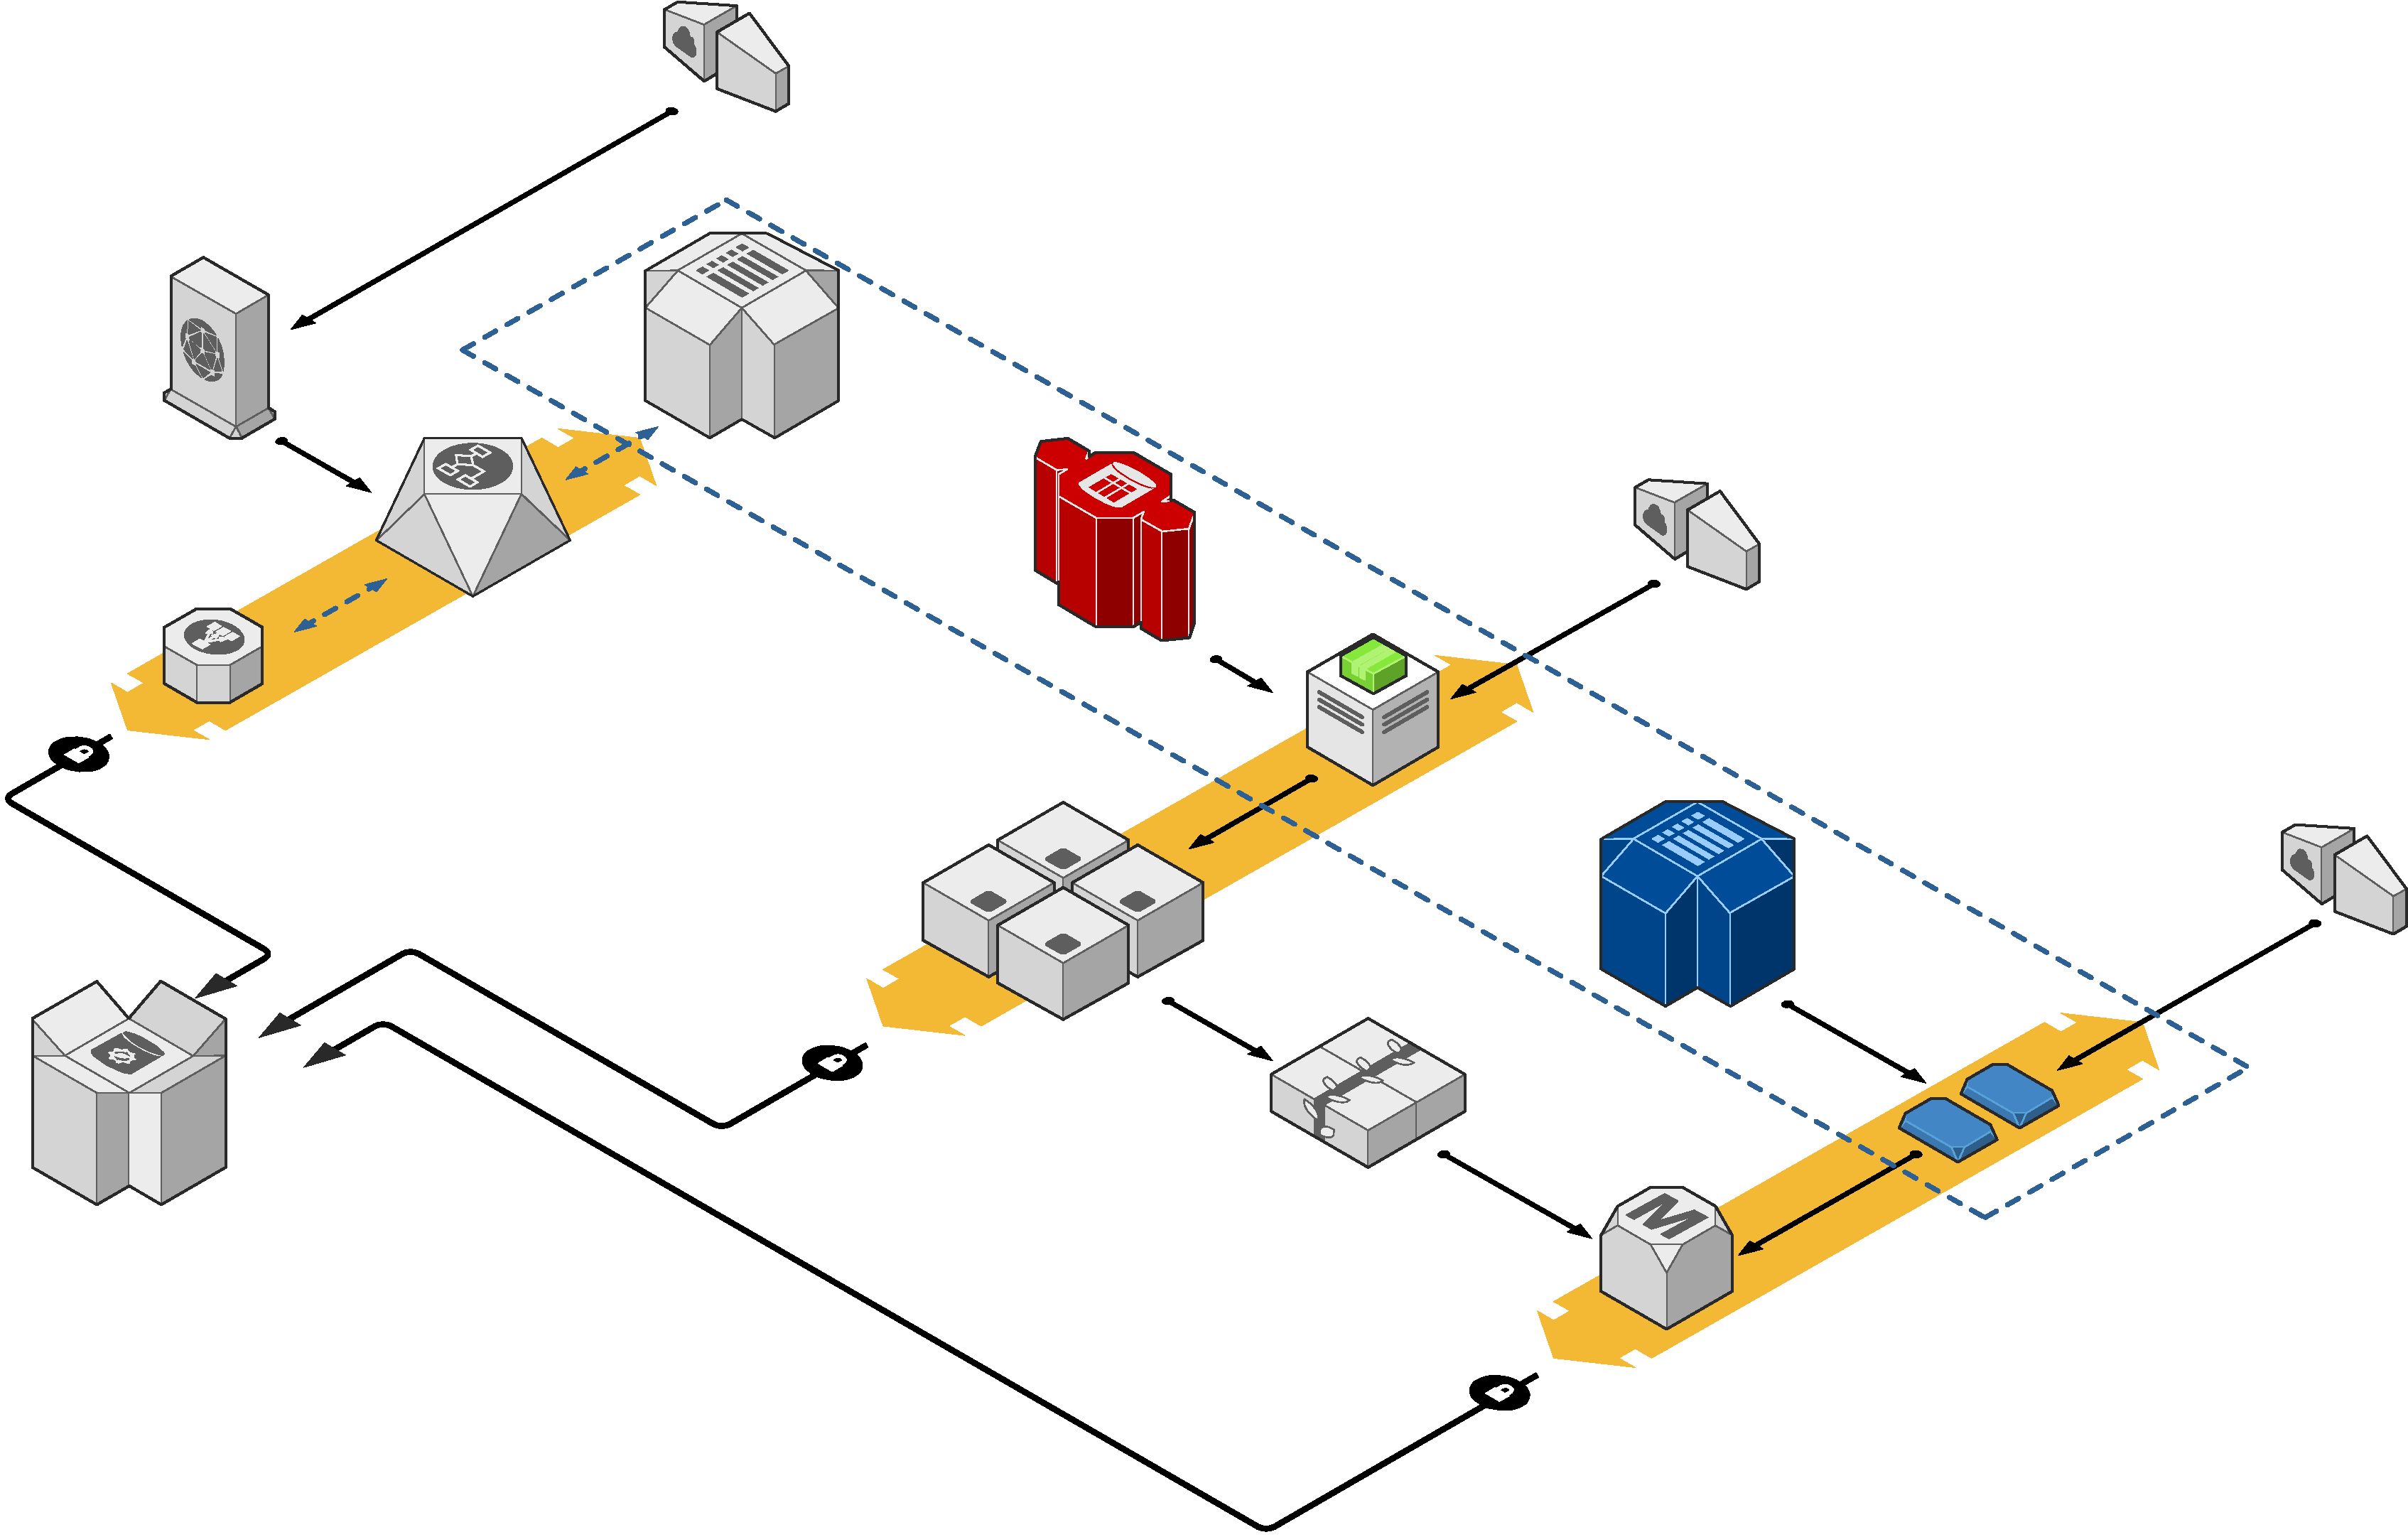
\includegraphics[width=\linewidth, bb=0 0 1626 1038]{example.pdf}
\caption{A really informative diagram following the magical-number-7-principle of Miller \cite{magical_2020}.}\label{fig:example-single}
\end{figure}

\noindent As shown in \Cref{fig:example-single}, including graphics is really easy with PDF files, but you need to give it a \textit{bounding box}, which is simply \texttt{0 0 <width> <height>}. Here is how to include PNG files.

\begin{figure}[H]
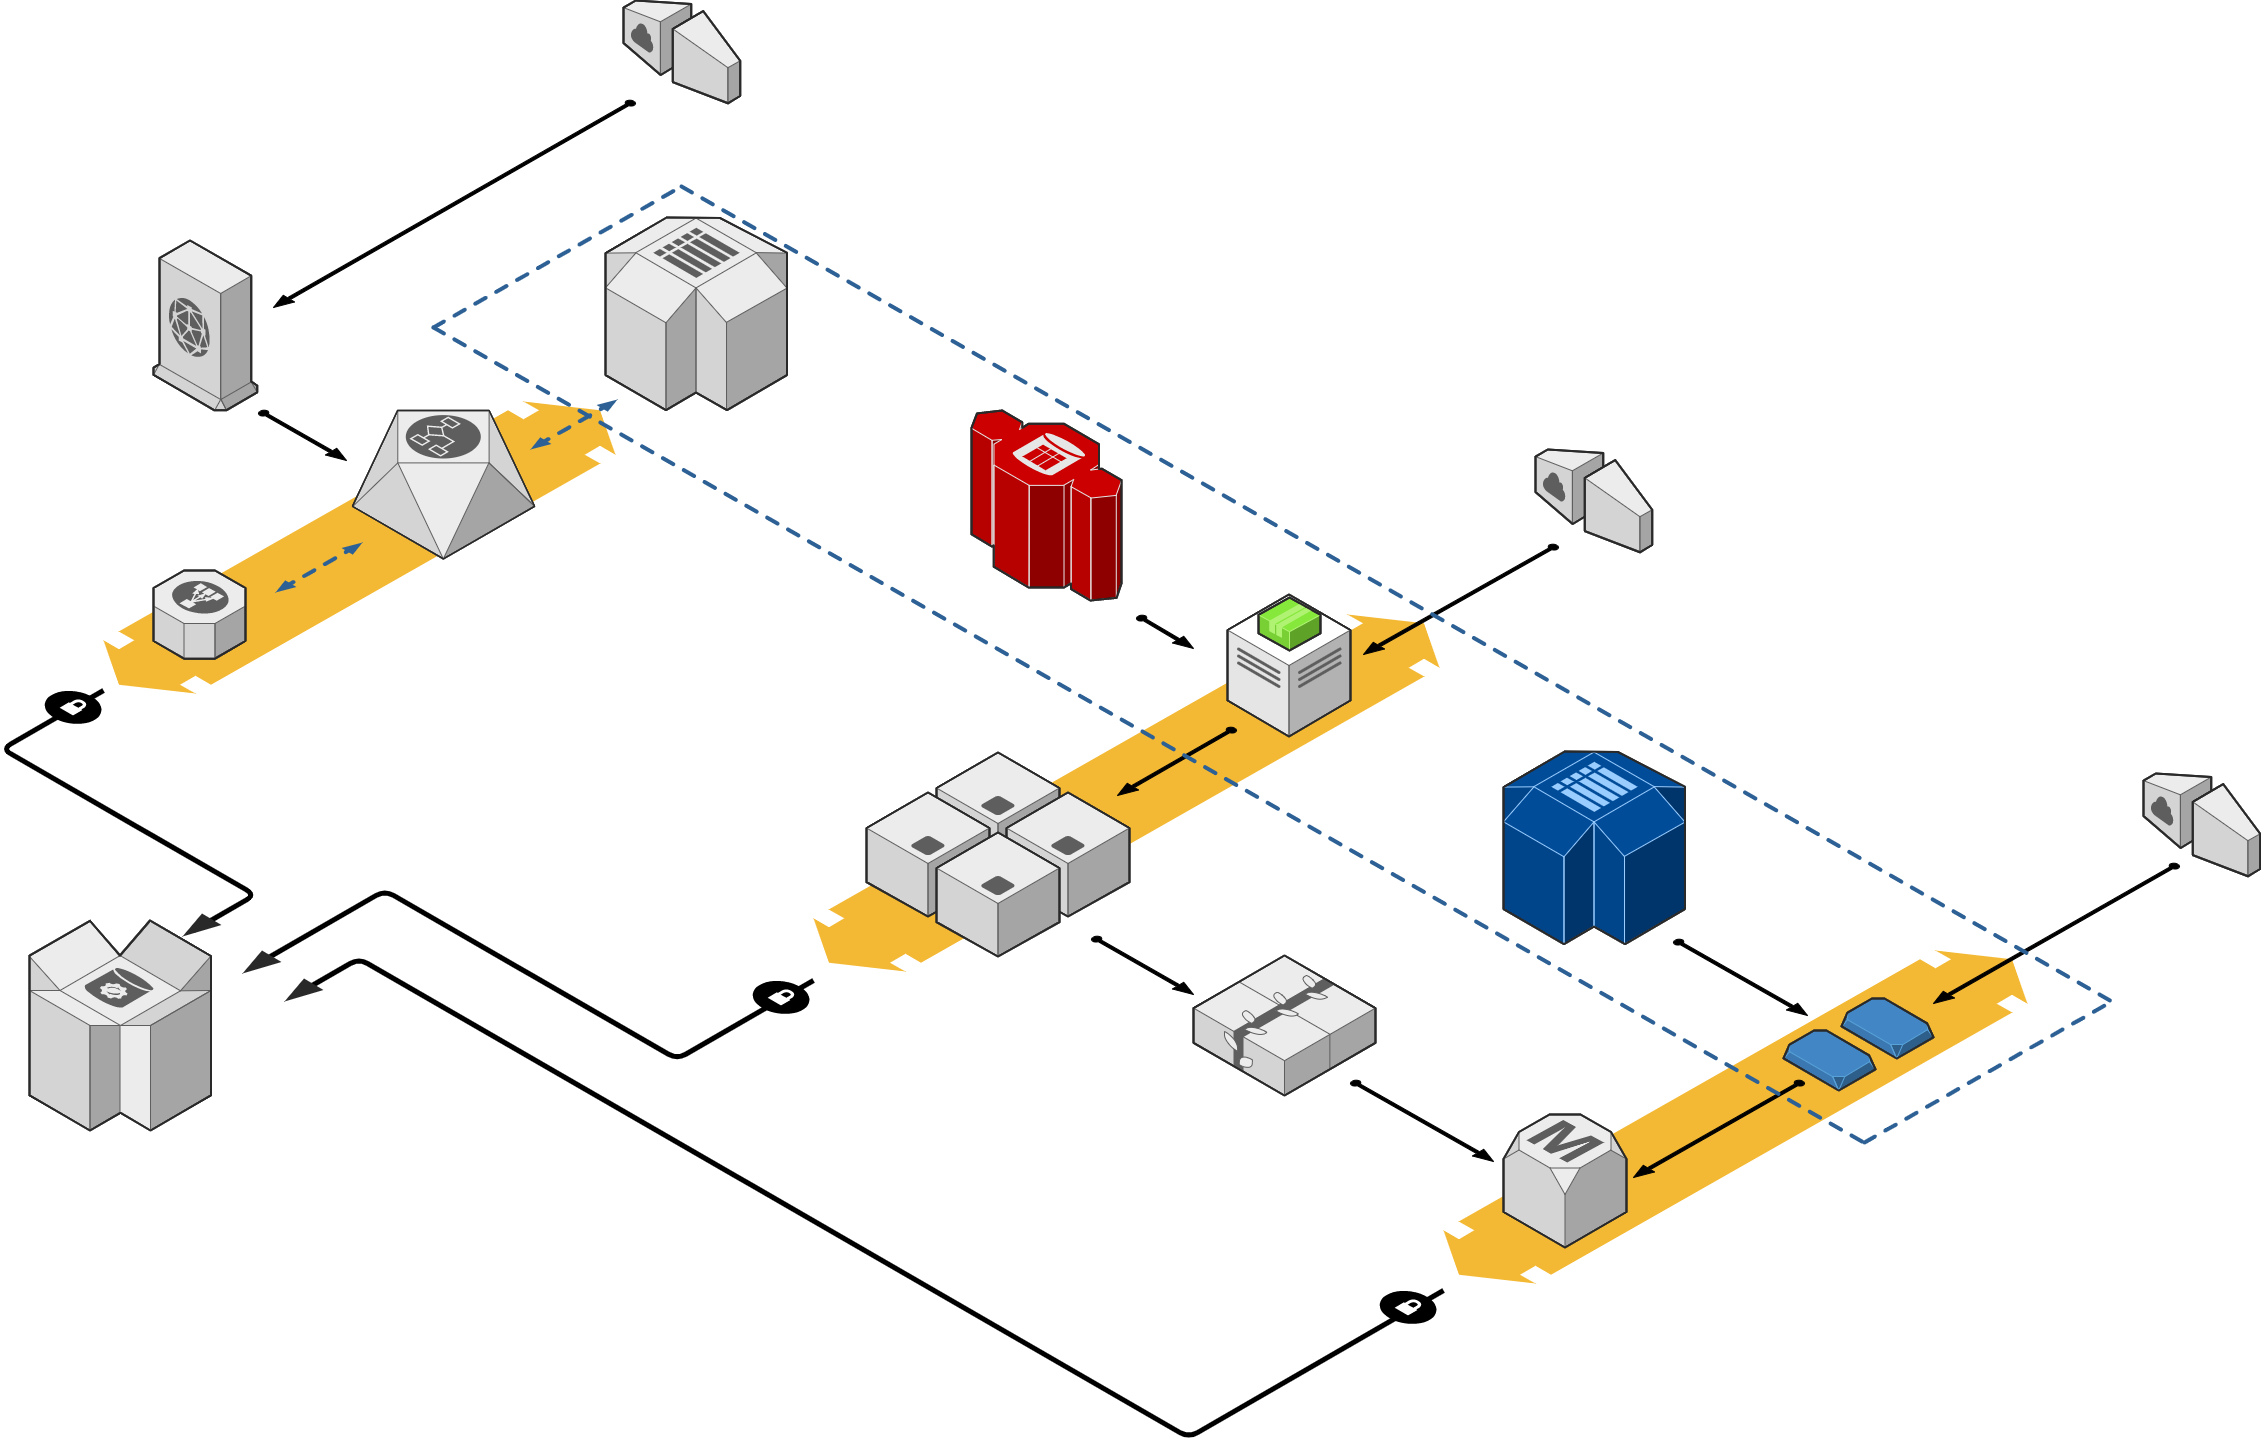
\includegraphics[width=0.75\linewidth]{example.png}
\caption{The same diagram but in PNG and smaller.}\label{fig:example-small}
\end{figure}

\noindent With PNG, no bounding box must be given, but the size of your thesis PDF will probably increase by some order of magnitudes. So try to use PDF whenever possible. Also, avoid JPEG because of the lossy compression. We want our thesis to look nice, or wont we? Try to fiddle around with the option \texttt{H} after the figure, if it doesn't fit the page. This will not be explained here, read the documentation.

\paragraph{One last example:} use the following snippet to include multiple graphics in a table-like structure.

\begin{figure}[H]
\begin{tabular}{ll}
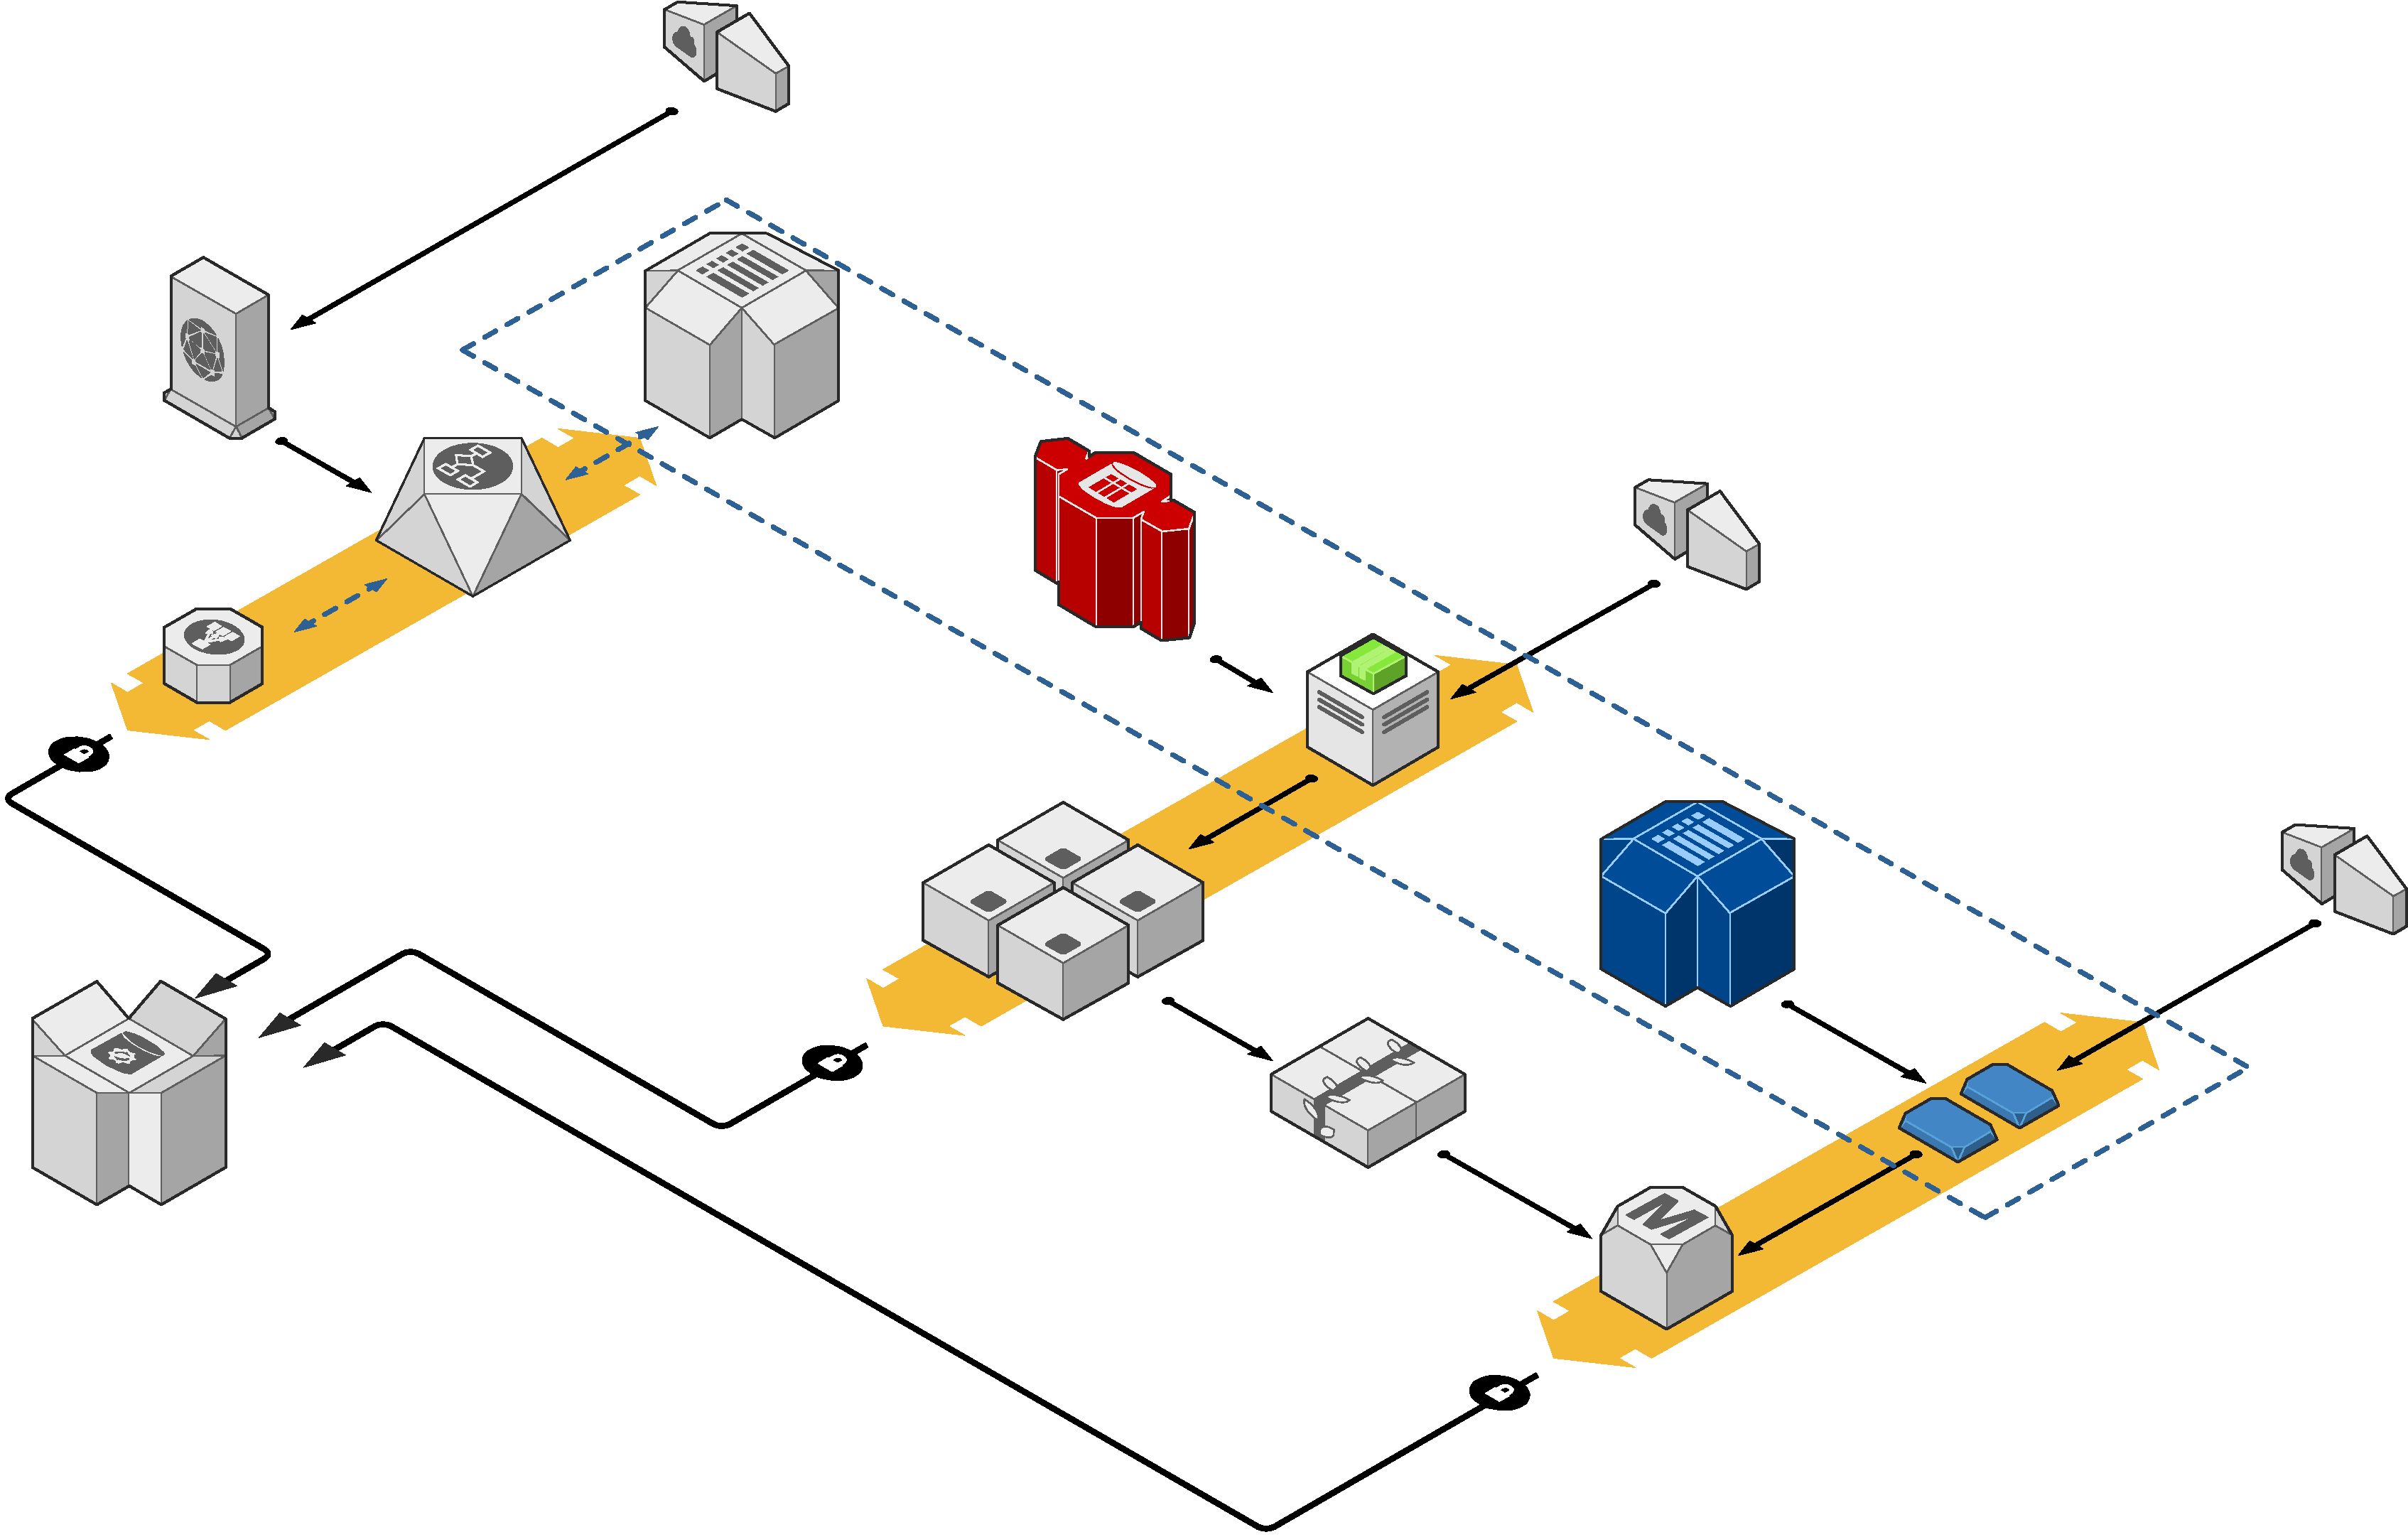
\includegraphics[width=0.4\linewidth, bb=0 0 1626 1038]{example.pdf}
&
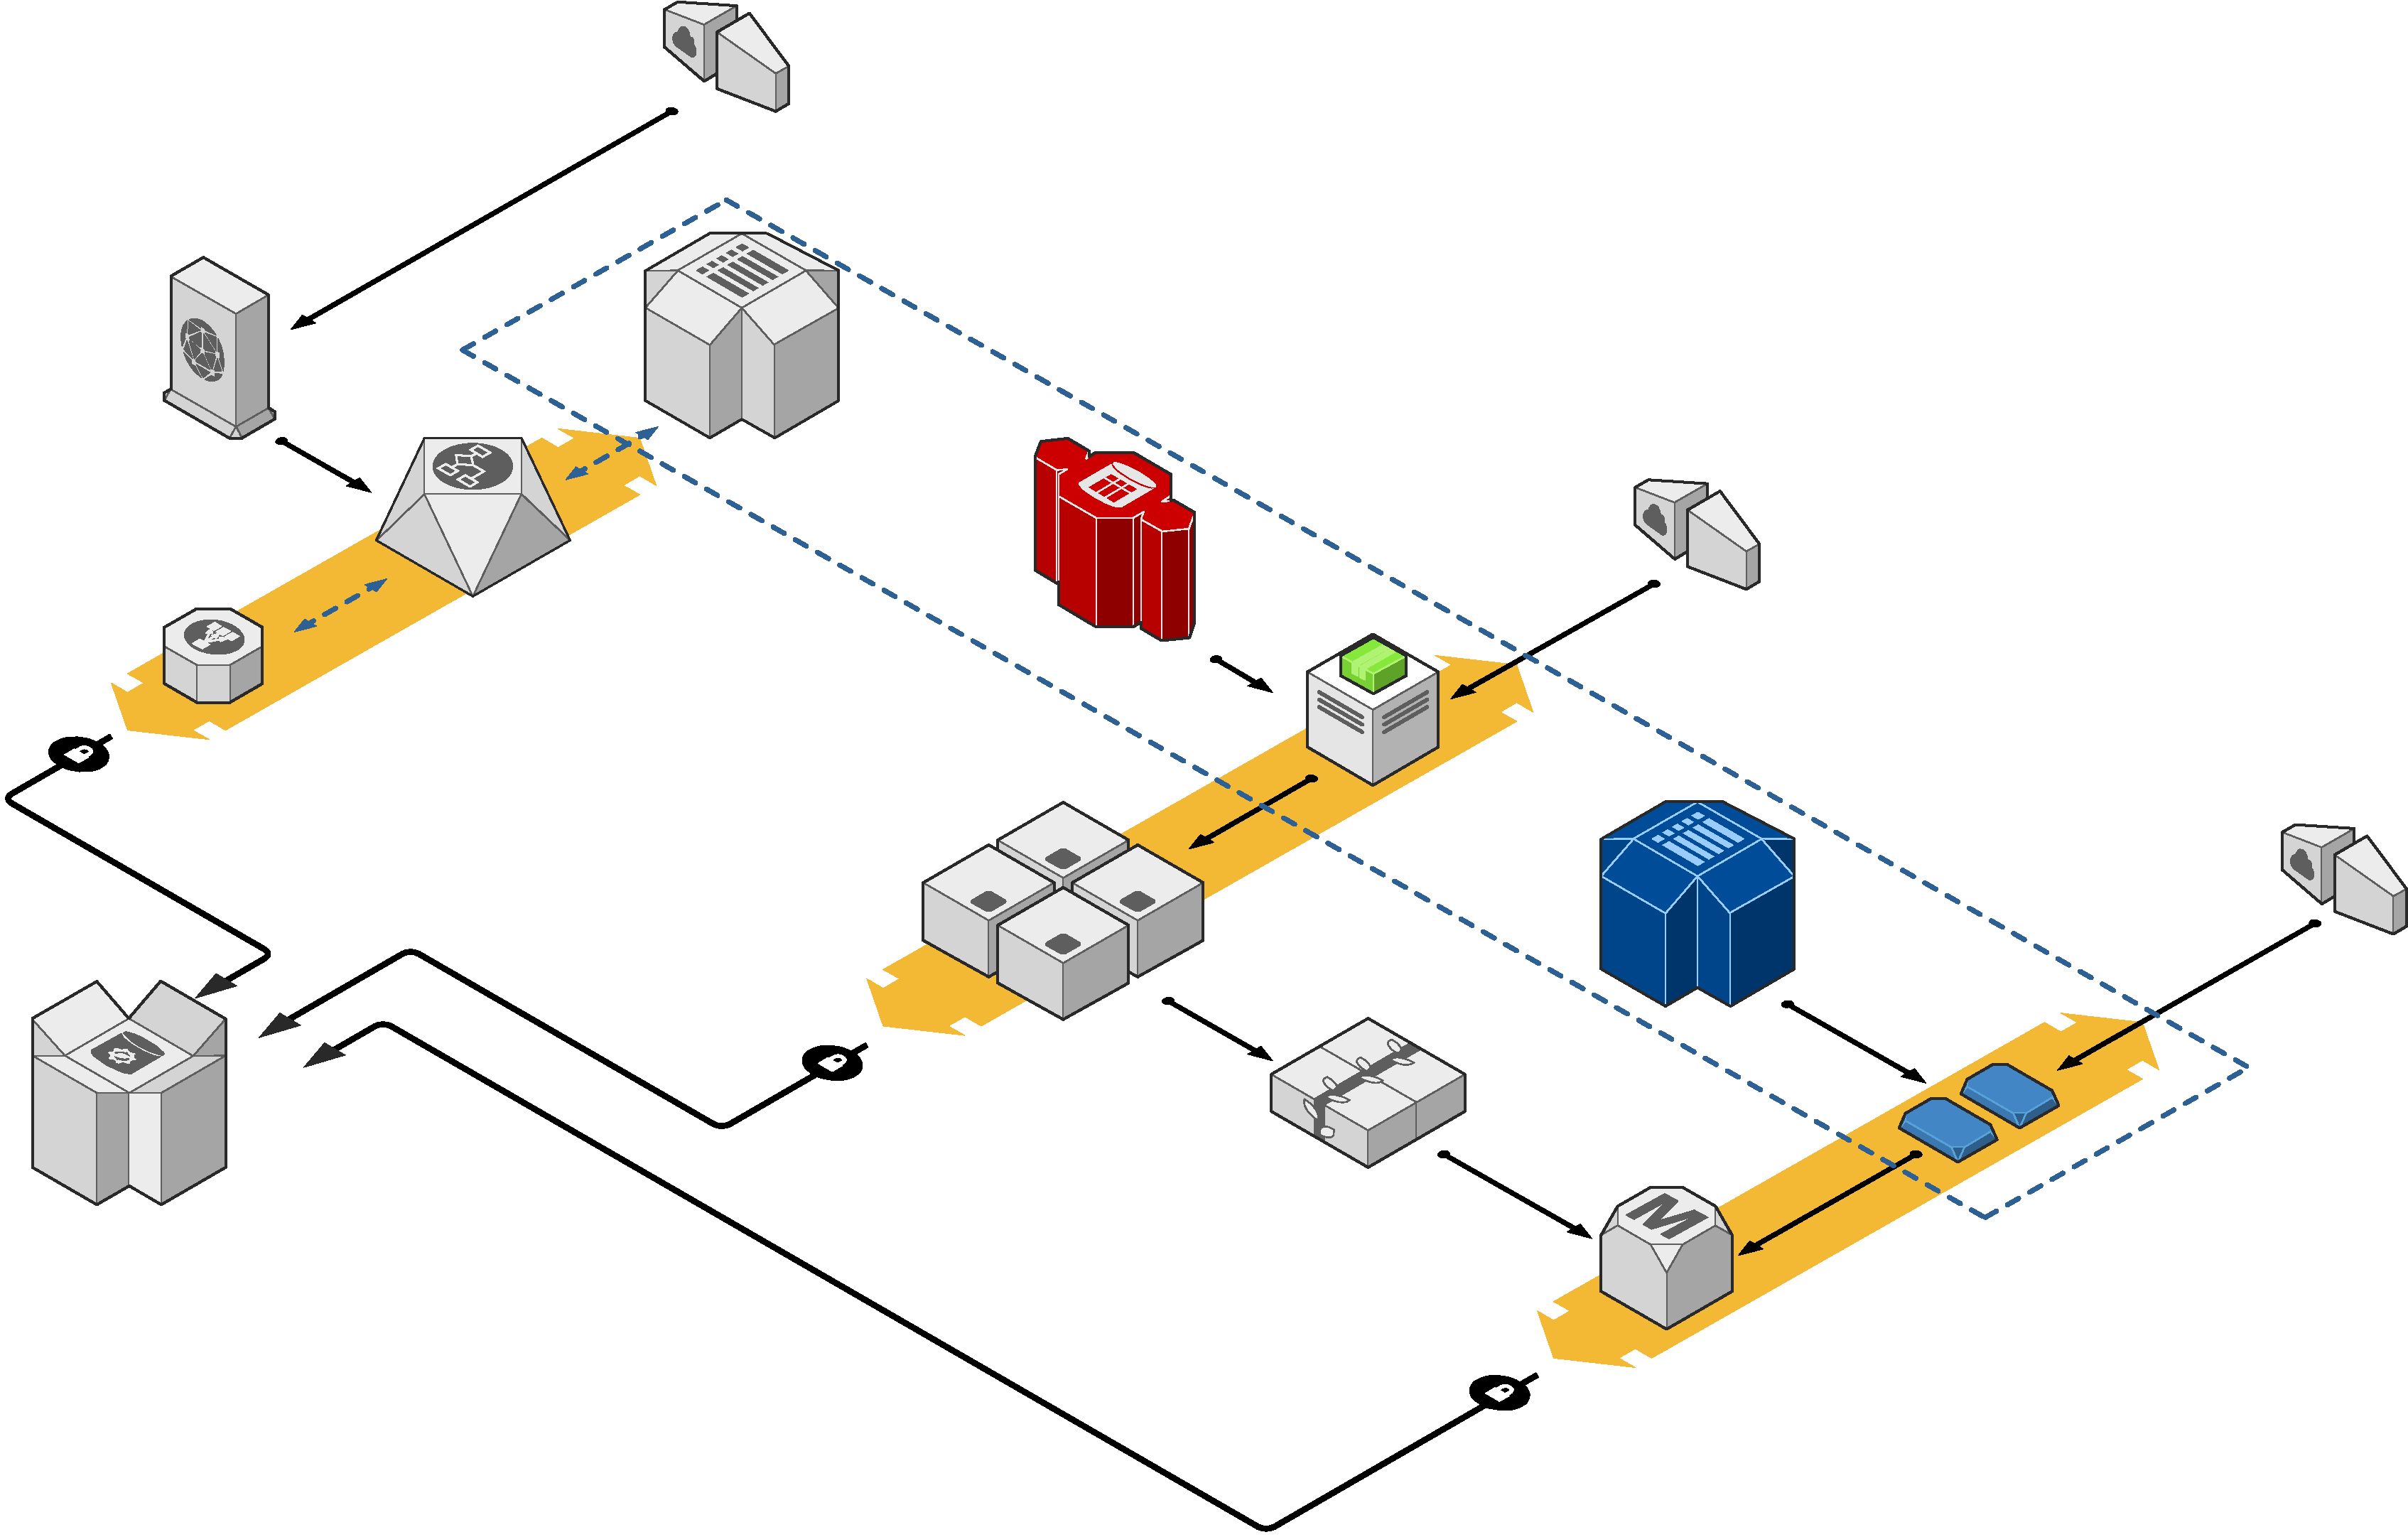
\includegraphics[width=0.4\linewidth, bb=0 0 1626 1038]{example.pdf}
\\
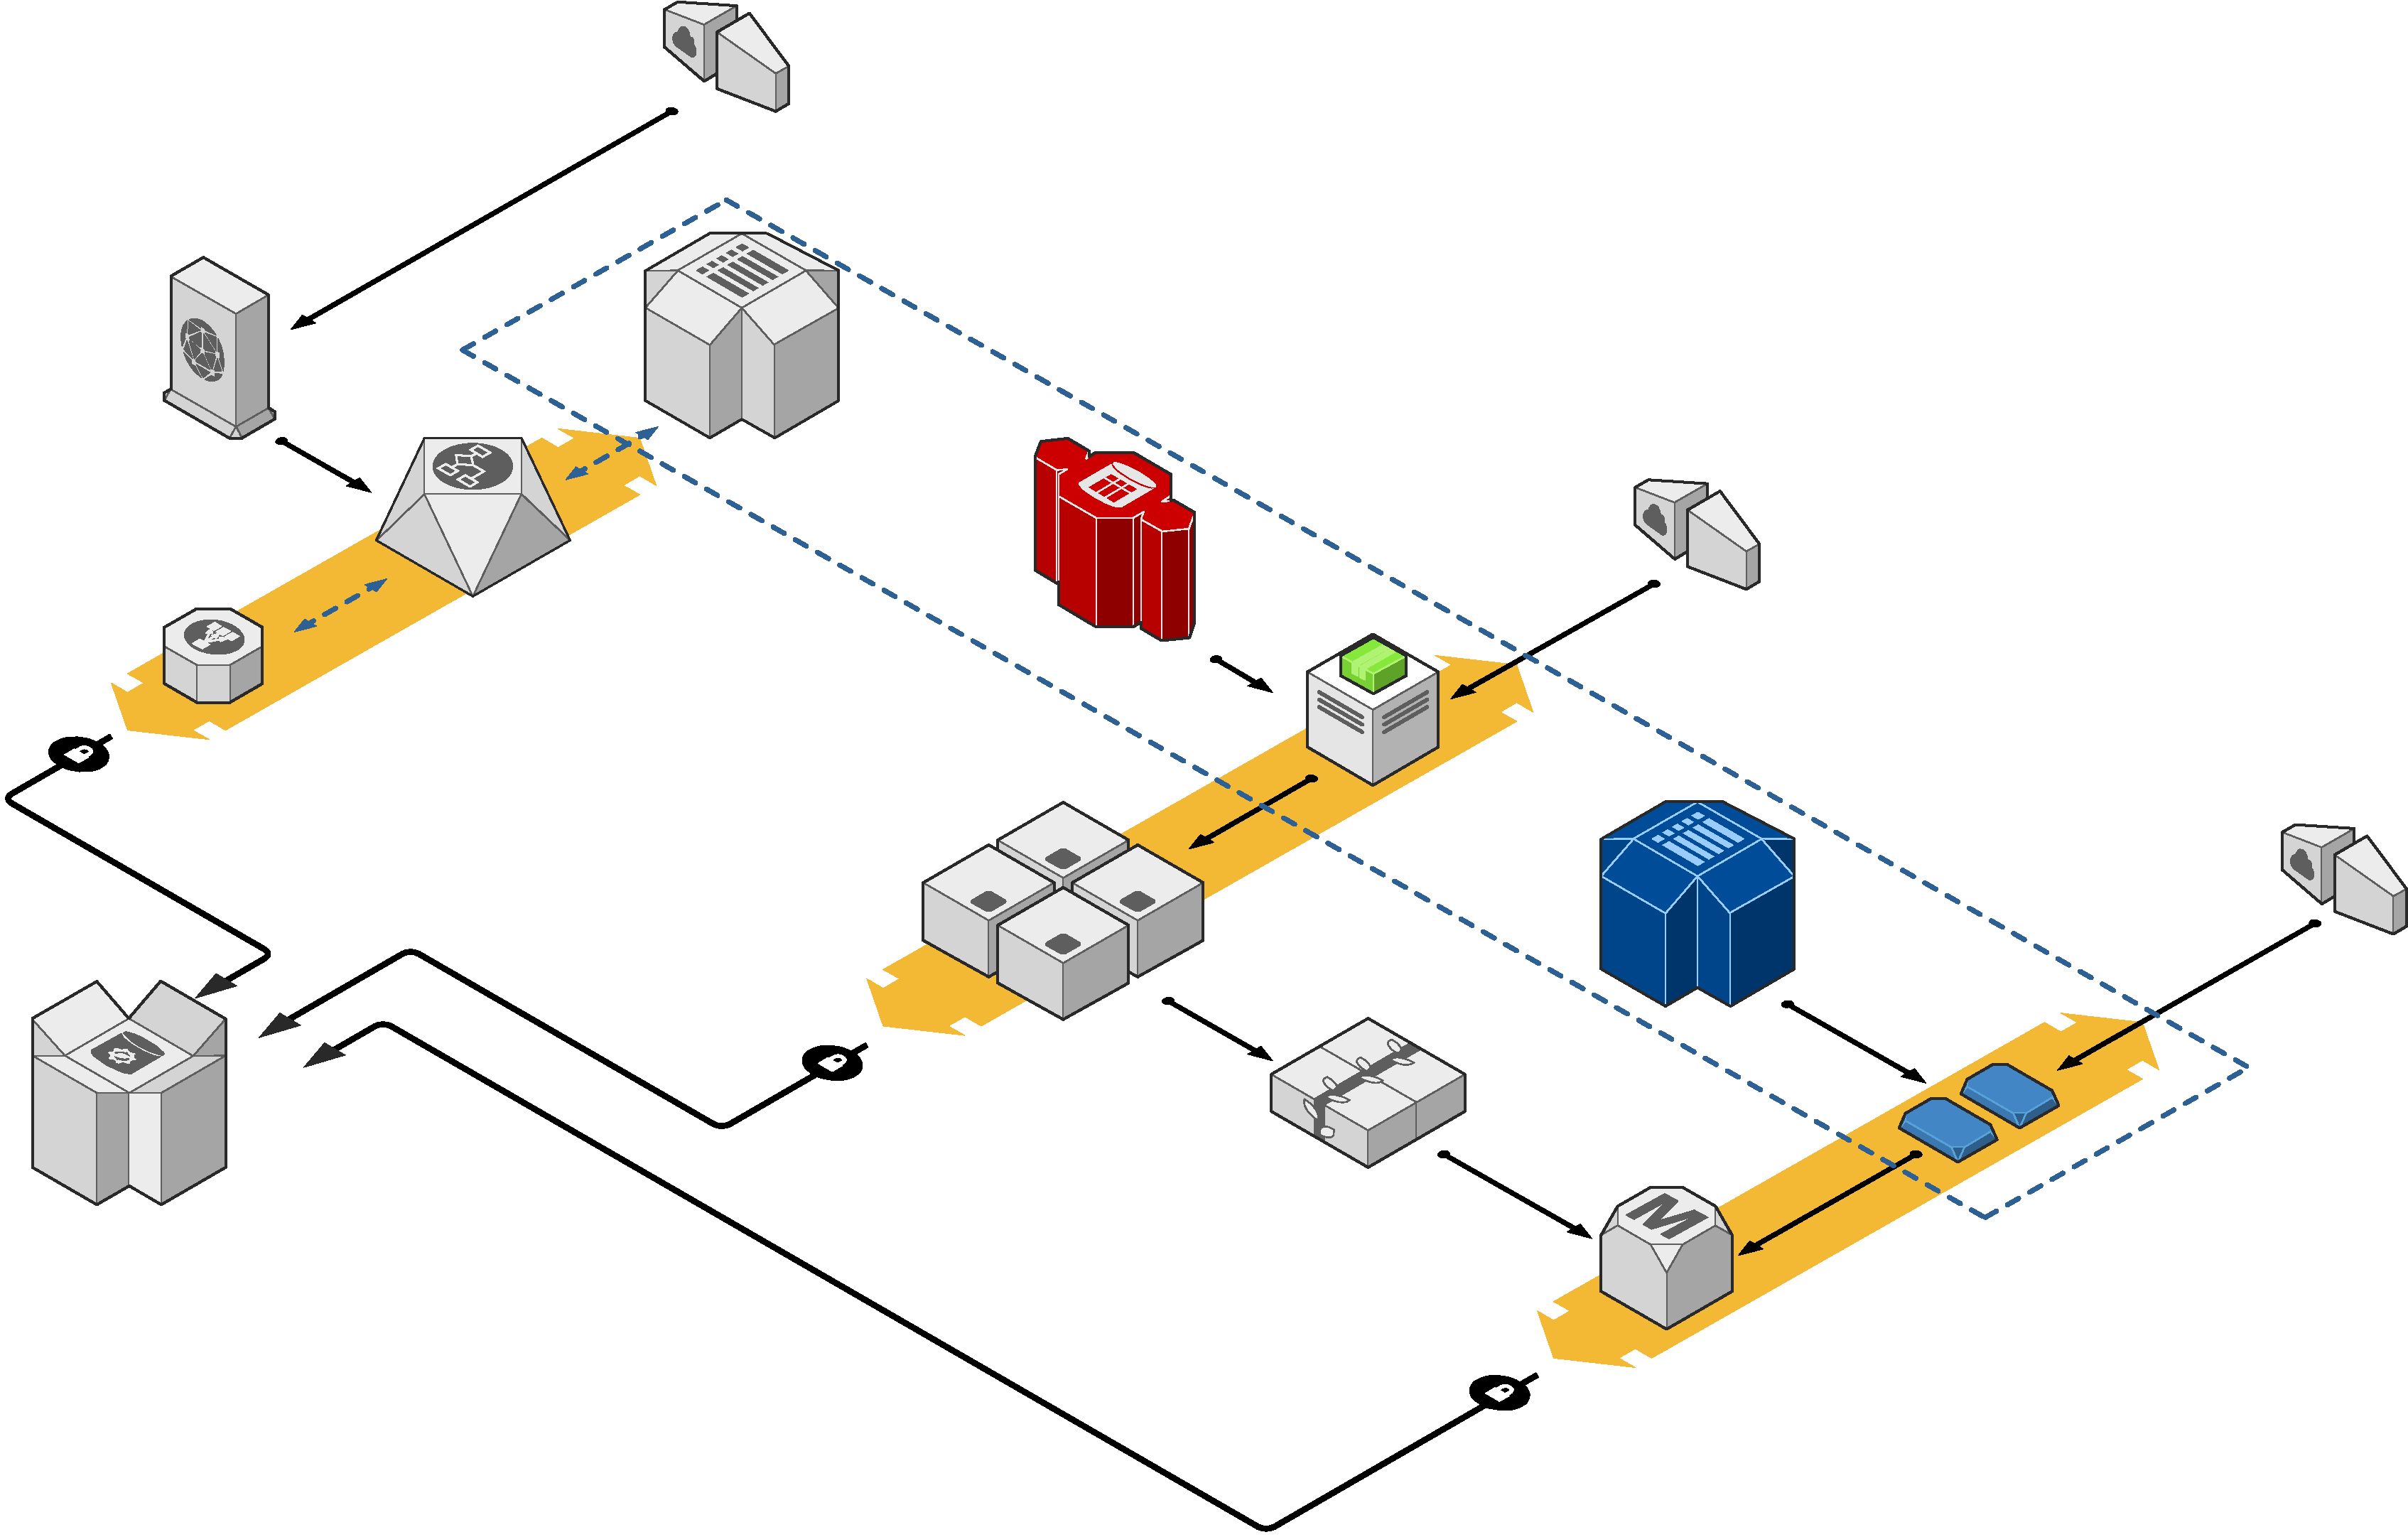
\includegraphics[width=0.4\linewidth, bb=0 0 1626 1038]{example.pdf}
&
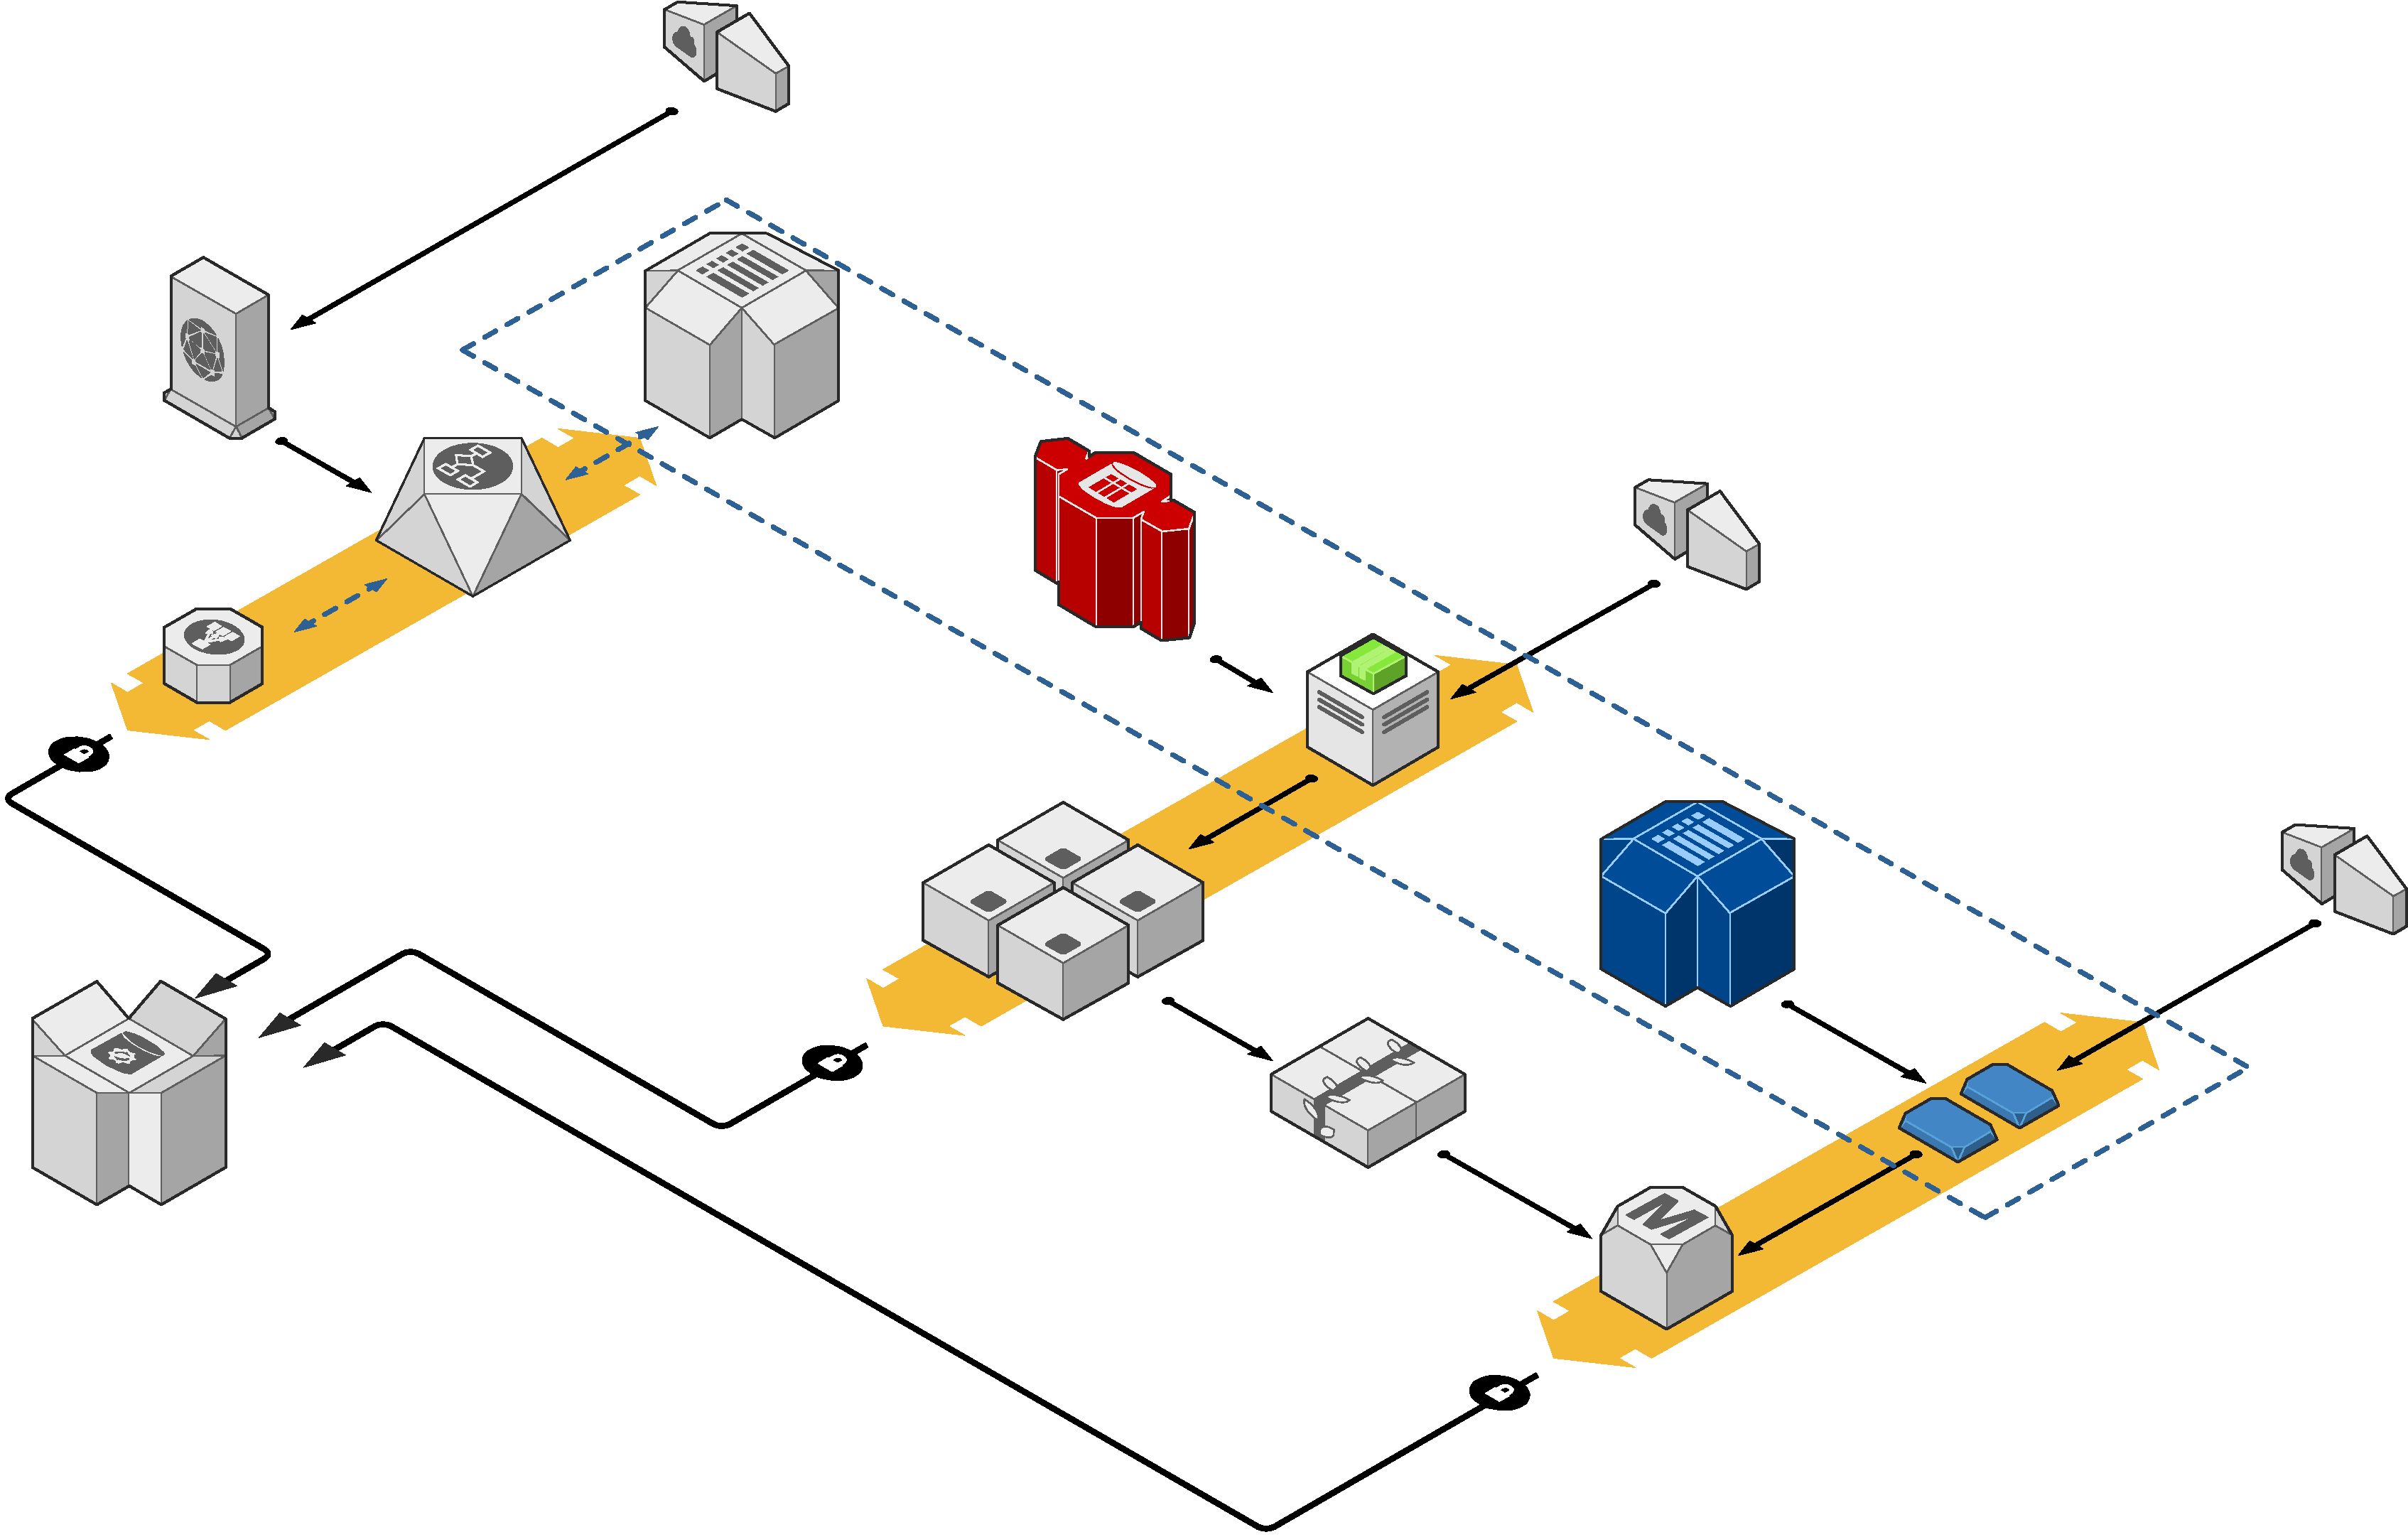
\includegraphics[width=0.4\linewidth, bb=0 0 1626 1038]{example.pdf}
\end{tabular}
\caption{Deja vu? It seems, like I've already seen this diagram.}\label{fig:example-multiple}
\end{figure}

\section{Code, Tables and Quotation}

What about some nice XML? Btw, always \enquote{quote} with the according tag.

\begin{lstlisting}[language=XML]
<note>
  <from>Philipp</from>
  <to>Reader</to>
  <heading>Contact me</heading>
  <email>mail@philippmatth.es</email>
</note>
\end{lstlisting}

\noindent Check out this table! Btw, this may seem a bit confusing, but there is \texttt{tabular}, \texttt{tabularx} or for example also \texttt{longtable}, which is for tables across multiple pages.

\begin{table}[H]
\caption{The caption of your table.}\label{tab:example}
\begin{tabularx}{\textwidth}{{
  >{\hsize=.5\hsize\linewidth=\hsize}X
  >{\hsize=1.5\hsize\linewidth=\hsize}X
}}
\hline
Column 1 & Wider Column 2 \\ \hline \hline
Entry 1.1 & Entry 1.2 \\ \hline
\end{tabularx}
\end{table}

\noindent This was nice. Is there anything missing? File a pull request!
